% ============================================================================
% Week 2-3 -- LECTURE NOTE (student-facing)
%
% Remainder of week 1 (IPs, relax-and-round, knapsack) + the week-2
% binary-variable toolbox. Style of week01-note.tex, condensed to board
% fragments. Self-contained -- no \input{preamble}.
% ============================================================================
\documentclass[10pt]{article}

\usepackage[a4paper, margin=1.5cm]{geometry}
\usepackage{amsmath, amssymb}
\usepackage[dvipsnames]{xcolor}
\usepackage{graphicx}
\usepackage{array}
\usepackage{tikz}
\usepackage{kotex}
\usepackage[hidelinks]{hyperref}

\definecolor{ruleink}{RGB}{18, 68, 140}
\definecolor{demoink}{RGB}{140, 82, 20}
\definecolor{keyink}{RGB}{20, 90, 20}
\definecolor{watchink}{RGB}{86, 60, 140}
\definecolor{punchink}{RGB}{170, 30, 60}

\setlength{\parindent}{0pt}
\pagestyle{empty}

% tighter spacing around centered displays
\AtBeginDocument{%
  \abovedisplayskip=4pt plus 1pt
  \belowdisplayskip=4pt plus 1pt
  \abovedisplayshortskip=2pt
  \belowdisplayshortskip=2pt}

% ---- one section -----------------------------------------------------------
\newcommand{\beat}[2]{%   number, title
  \par\medskip
  {\color{ruleink}\rule{\textwidth}{1pt}}\par\nobreak\vspace{2pt}
  {\large\bfseries #1.\; #2}\par\nobreak\vspace{3pt}}

% ---- board content ---------------------------------------------------------
\newenvironment{board}{%
  \par\vspace{2pt}
  \begingroup\leftskip=1.3em\relax}{%
  \par\endgroup\vspace{2pt}}

% ---- highlights ------------------------------------------------------------
\newcommand{\demo}[2]{\par{\color{demoink}\small\textbf{demo}\quad\texttt{#1} --- #2}\par}
\newcommand{\watch}[1]{\par{\color{watchink}\small\textbf{watch}\quad #1}\par}
\newcommand{\key}[1]{\par\vspace{1pt}{\color{keyink}\small\textbf{KEY}\quad\textbf{#1}}\par}
\newcommand{\takeaway}[1]{%
  \par\vspace{2pt}\noindent
  {\color{punchink}\rule{2pt}{10pt}}\;{\color{punchink}\small\textbf{takeaway}\quad\textbf{#1}}\par\vspace{2pt}}

\begin{document}

{\Large\bfseries Week 2 --- Integer Programs and the Binary-Variable Toolbox}\\[2pt]
{\small OL7014 Integer Programming \quad\textbullet\quad Instructor: Prof.\ H.\ Park \quad\textbullet\quad Week of Aug 31, 2026}

% ---------------------------------------------------------------- 1
\beat{1}{Integer Programming (IP): add integrality --- and lose convexity}
\begin{board}
one new line on last week's LP: \qquad $x, y \in \mathbb{Z}$
\[
  X \;=\; P \cap \mathbb{Z}^n
  \qquad\quad P = \{\, x : Ax \le b \,\} = \text{linear container (last week's polyhedron)}, \quad X = \text{lattice points inside}
\]
\emph{read the symbols:} \quad $\mathbb{Z}$ = the integers, \quad $\cap$ = intersection (points in \emph{both} sets)
\vspace{3pt}

\textbf{pure IP}:
\[
\begin{aligned}
  \max_{x}\quad & c^{\top}x \\
  \text{s.t.}\quad & Ax \le b \\
                   & x \in \mathbb{Z}^n
\end{aligned}
\]
\textbf{binary program (BP)} --- every decision a yes/no switch:
\[
\begin{aligned}
  \max_{x}\quad & c^{\top}x \\
  \text{s.t.}\quad & Ax \le b \\
                   & x \in \{0,1\}^n \quad (\text{or } x \in \mathbb{B}^n)
\end{aligned}
\]
\quad $x_j \in \{0,1\}$ or $x_j \in \mathbb{B}$; \quad
$x_j \in \{0,1\} \iff x_j \in \mathbb{Z}, \ 0 \le x_j \le 1$ \quad --- a BP is an IP with $0/1$ bounds
\vspace{4pt}

\textbf{mixed-integer LP (MILP)} --- integer $x$ and continuous $y$ mixed:
\[
\begin{aligned}
  \max_{x,\,y}\quad & c^{\top}x + h^{\top}y \\
  \text{s.t.}\quad & Ax + Gy \le b \\
                   & x \in \mathbb{Z}^n_{+}, \quad y \ge 0
\end{aligned}
\]
\vspace{1pt}

\quad \emph{example:} \ last week's toy with crates integer ($x_1$ = ammo, $x_2$ = rations),
plus fuel $y$ (liters --- divisible):
\[
\begin{aligned}
  \max\quad & 4x_1 + 5x_2 + 2y \\
  \text{s.t.}\quad & x_1 + 3x_2 + y \le 10 \\
                   & 3x_1 + x_2 + 2y \le 10 \\
                   & x \in \mathbb{Z}^2_{+}, \quad y \ge 0
\end{aligned}
\]
\quad $(c, A, b)$ we already know --- the \emph{only} new pieces are $h$ and $G$:
\[
  c = \begin{pmatrix} 4 \\ 5 \end{pmatrix}, \qquad
  A = \begin{pmatrix} 1 & 3 \\ 3 & 1 \\ -1 & 0 \\ 0 & -1 \end{pmatrix}, \qquad
  h = \begin{pmatrix} 2 \end{pmatrix}, \qquad
  G = \begin{pmatrix} 1 \\ 2 \\ 0 \\ 0 \end{pmatrix}, \qquad
  b = \begin{pmatrix} 10 \\ 10 \\ 0 \\ 0 \end{pmatrix}
\]
\quad (rows 3--4 are $x \ge 0$, exactly as last week; $y \ge 0$ comes with the form)
\vspace{3pt}

\textbf{$X$ is \emph{not} convex} --- midpoint of two lattice points need not be one
\end{board}
\key{convention: $x$ integer decisions, $y$ continuous.}
\begin{center}
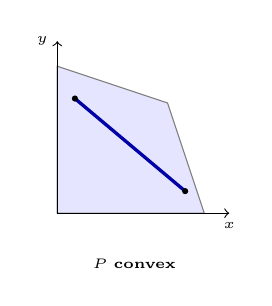
\begin{tikzpicture}[scale=0.56, font=\tiny]
  \fill[blue!10] (0,0) -- (10/3,0) -- (2.5,2.5) -- (0,10/3) -- cycle;
  \draw[thin,gray] (0,0) -- (10/3,0) -- (2.5,2.5) -- (0,10/3) -- cycle;
  \draw[->] (0,0) -- (3.9,0) node[below] {$x$}; \draw[->] (0,0) -- (0,3.9) node[left] {$y$};
  \draw[very thick, blue!65!black] (0.4,2.6) -- (2.9,0.5);
  \fill (0.4,2.6) circle (2pt); \fill (2.9,0.5) circle (2pt);
  \node[align=center] at (1.75,-1.15) {$P$ \textbf{convex}};
\end{tikzpicture}
\hspace{10mm}
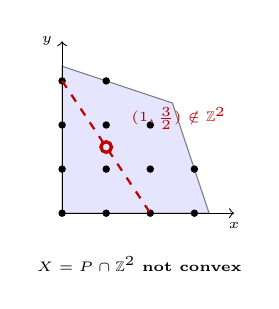
\begin{tikzpicture}[scale=0.56, font=\tiny]
  \fill[blue!10] (0,0) -- (10/3,0) -- (2.5,2.5) -- (0,10/3) -- cycle;
  \draw[thin,gray] (0,0) -- (10/3,0) -- (2.5,2.5) -- (0,10/3) -- cycle;
  \draw[->] (0,0) -- (3.9,0) node[below] {$x$}; \draw[->] (0,0) -- (0,3.9) node[left] {$y$};
  \foreach \p in {(0,0),(1,0),(2,0),(3,0),(0,1),(1,1),(2,1),(3,1),(0,2),(1,2),(2,2),(0,3),(1,3)}
    \fill \p circle (2.4pt);
  \draw[dashed, red!75!black, thick] (0,3) -- (2,0);
  \draw[red!75!black, very thick] (1,1.5) circle (3.4pt);
  \node[red!75!black, anchor=west, font=\tiny] at (1.35,2.15) {$(1,\tfrac{3}{2}) \notin \mathbb{Z}^2$};
  \node[align=center] at (1.75,-1.15) {$X = P \cap \mathbb{Z}^2$ \textbf{not convex}};
\end{tikzpicture}
\end{center}

\begin{center}
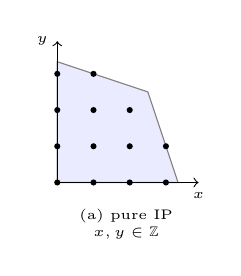
\begin{tikzpicture}[scale=0.46, font=\tiny]
  \fill[blue!8] (0,0) -- (10/3,0) -- (2.5,2.5) -- (0,10/3) -- cycle;
  \draw[thin,gray] (0,0) -- (10/3,0) -- (2.5,2.5) -- (0,10/3) -- cycle;
  \draw[->] (0,0) -- (3.9,0) node[below] {$x$}; \draw[->] (0,0) -- (0,3.9) node[left] {$y$};
  \foreach \p in {(0,0),(1,0),(2,0),(3,0),(0,1),(1,1),(2,1),(3,1),(0,2),(1,2),(2,2),(0,3),(1,3)}
    \fill \p circle (2.4pt);
  \node[align=center] at (1.9,-1.15) {(a) pure IP\\ $x,y \in \mathbb{Z}$};
\end{tikzpicture}\hspace{7mm}
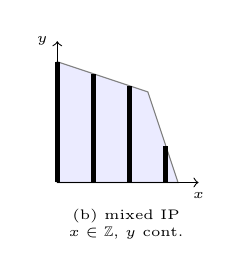
\begin{tikzpicture}[scale=0.46, font=\tiny]
  \fill[blue!8] (0,0) -- (10/3,0) -- (2.5,2.5) -- (0,10/3) -- cycle;
  \draw[thin,gray] (0,0) -- (10/3,0) -- (2.5,2.5) -- (0,10/3) -- cycle;
  \draw[->] (0,0) -- (3.9,0) node[below] {$x$}; \draw[->] (0,0) -- (0,3.9) node[left] {$y$};
  \draw[line width=1.8pt] (0,0) -- (0,10/3); \draw[line width=1.8pt] (1,0) -- (1,3);
  \draw[line width=1.8pt] (2,0) -- (2,8/3); \draw[line width=1.8pt] (3,0) -- (3,1);
  \node[align=center] at (1.9,-1.15) {(b) mixed IP\\ $x \in \mathbb{Z}$, $y$ cont.};
\end{tikzpicture}\hspace{7mm}
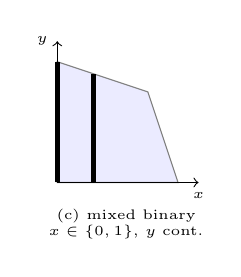
\begin{tikzpicture}[scale=0.46, font=\tiny]
  \fill[blue!8] (0,0) -- (10/3,0) -- (2.5,2.5) -- (0,10/3) -- cycle;
  \draw[thin,gray] (0,0) -- (10/3,0) -- (2.5,2.5) -- (0,10/3) -- cycle;
  \draw[->] (0,0) -- (3.9,0) node[below] {$x$}; \draw[->] (0,0) -- (0,3.9) node[left] {$y$};
  \draw[line width=1.8pt] (0,0) -- (0,10/3); \draw[line width=1.8pt] (1,0) -- (1,3);
  \node[align=center] at (1.9,-1.15) {(c) mixed binary\\ $x \in \{0,1\}$, $y$ cont.};
\end{tikzpicture}\\[2pt]
{\footnotesize same $P$ --- what changes is \emph{which points you may use}}
\end{center}
\takeaway{one line, $\in \mathbb{Z}$, throws convexity away --- the whole course is the bill for that line.}

% ---------------------------------------------------------------- 2
\beat{2}{Why ``relax and round'' fails}
\begin{board}
\textbf{LP relaxation}: delete $x \in \mathbb{Z}^n$ \ $\Rightarrow$ \ optimize over $P$ instead of $X$
\vspace{3pt}

toy problem: LP optimum $(2.5,\,2.5)$, $z = 22.5$ --- just round it? \ $2^2 = 4$ candidates:
\vspace{3pt}

\begin{center}
\begin{tabular}{c|c|c|c}
 candidate & $x+3y \le 10$ & $3x+y \le 10$ & $z = 4x+5y$ \\ \hline
 $(2,2)$ & $8$ \checkmark & $8$ \checkmark & $18$ \\
 $(3,2)$ & $9$ \checkmark & $11$ $\times$ & infeasible \\
 $(2,3)$ & $11$ $\times$ & --- & infeasible \\
 $(3,3)$ & $12$ $\times$ & --- & infeasible \\
\end{tabular}
\end{center}

but: \quad $(1,\,3)$: \ $10$ \checkmark, \ $6$ \checkmark, \ $z = \mathbf{19}$
\[
  \underbrace{z_{\mathrm{LP}} = 22.5}_{\text{bound}} \;\;\ge\;\;
  \underbrace{z_{\mathrm{IP}} = 19}_{\text{optimum, at }(1,3)} \;\;>\;\;
  \underbrace{18}_{\text{best rounding}}
\]
\end{board}
\key{\begin{tabular}[t]{@{}l@{}}
1. rounding loses \emph{feasibility} and \emph{optimality} --- in $n$ dims, all $2^n$ candidates can die. \\
2. integrality changes \emph{where} the answer is. \\
3. but $z_{\mathrm{LP}} \ge z_{\mathrm{IP}}$ \emph{always} --- deleting a constraint only enlarges the feasible set.
\end{tabular}}
\demo{demo1\_toy\_ip.py}{drag $c_2$: the IP optimum \emph{hops}; no rounding rule predicts the hops.}
\takeaway{the relaxation gives not the answer but a \emph{bound} --- and bounds are how every IP is actually solved.}

% ---------------------------------------------------------------- 3
\beat{3}{Knapsack --- play it, then formulate it}
\demo{ip-games / knapsack}{play FIRST: rucksack, 21 kg, six items. \ \url{https://hankpark0706.github.io/ip-games/knapsack.html}}
\begin{board}
\begin{center}
\begin{tabular}{l|cccccc}
 item        & rifle & boots & helmet & canteen & med kit & rations \\ \hline
 weight (kg) & 5 & 7 & 8 & 8 & 8 & 2 \\
 value (pts) & 9 & 8 & 9 & 8 & 3 & 9 \\
\end{tabular}
\qquad $W = 21$
\end{center}

$x_j = 1$ if item $j$ packed, $0$ if not \qquad --- a \emph{choice}, not a quantity
\[
\begin{aligned}
  \max\quad & \textstyle\sum_j v_j\, x_j \\
  \text{s.t.}\quad & \textstyle\sum_j w_j\, x_j \;\le\; W \\
                   & x_j \in \{0,1\} \ \ \forall j
\end{aligned}
\]
all variables binary $\Rightarrow$ a \textbf{binary program (BP)}
\vspace{4pt}

greedy (value/weight): \ rations, rifle, boots \ $= 26$ \ (14 kg)
\vspace{2pt}

optimum: \qquad\qquad\quad\ \ rations, rifle, helmet $= \mathbf{27}$ \ (15 kg)
\[
  \underbrace{33.875}_{\text{LP (bound)}} \;\;\ge\;\; \underbrace{27}_{\text{IP}} \;\;>\;\;
  \underbrace{26}_{\text{greedy \emph{and} rounded LP}}
\]
\end{board}
\key{one constraint, six variables --- already NP-hard.}
\takeaway{the optimum uses 15 kg of 21 --- integrality can leave capacity on the table.}

% ---------------------------------------------------------------- 4
\beat{4}{From scalar model to matrix form --- the rewriting dictionary}
\begin{board}
modeling = scalar lines; solving = matrices: Gurobi receives exactly $(c, h, A, G, b)$
\vspace{3pt}

first, one with numbers --- watch every move:
\[
\begin{aligned}
  \min\quad & x_1 - 2x_2 \\
  \text{s.t.}\quad & x_1 + x_2 \ge 3 \\
                   & x_1 - x_2 = 1 \\
                   & x_1 \ge 0, \quad x_2 \ \text{free}
\end{aligned}
\qquad\Longrightarrow\qquad
\begin{aligned}
  -\max\quad & -x_1 + 2u - 2v \\
  \text{s.t.}\quad & -x_1 - u + v \le -3 \\
                   & x_1 - u + v \le 1, \quad -x_1 + u - v \le -1 \\
                   & x_1,\, u,\, v \ge 0 \qquad (x_2 = u - v)
\end{aligned}
\]
\quad min flipped, $\ge$ flipped, $=$ split into two $\le$, free $x_2$ split into $u - v$ --- then read off:
\[
  c = \begin{pmatrix} -1 \\ 2 \\ -2 \end{pmatrix}, \qquad
  A = \begin{pmatrix} -1 & -1 & 1 \\ 1 & -1 & 1 \\ -1 & 1 & -1 \\ -1 & 0 & 0 \\ 0 & -1 & 0 \\ 0 & 0 & -1 \end{pmatrix}, \qquad
  b = \begin{pmatrix} -3 \\ 1 \\ -1 \\ 0 \\ 0 \\ 0 \end{pmatrix}
  \qquad \text{(last three rows are $x_1, u, v \ge 0$)}
\]
\vspace{3pt}

the general dictionary:
\begin{center}
\begin{tabular}{lll}
 you wrote & rewrite as & cost \\ \hline
 $\min\, c^{\top}x$ & $-\max\, (-c)^{\top}x$ & --- \\[2pt]
 $a^{\top}x \ge \beta$ & $-a^{\top}x \le -\beta$ & --- \\[2pt]
 $a^{\top}x = \beta$ & $a^{\top}x \le \beta$ \ and \ $-a^{\top}x \le -\beta$ & one row \\[2pt]
 $x_j$ free & $x_j = x_j^{+} - x_j^{-}$, \ $x_j^{+}, x_j^{-} \ge 0$ & one variable \\[2pt]
 bound $x_j \le u_j$ & one more row & one row \\[2pt]
 $x_j \in \{0,1\}$ & $x_j \in \mathbb{Z}$, \ $0 \le x_j \le 1$ & --- \\[2pt]
 $a^{\top}x \le \beta$, want $=$ & $a^{\top}x + s = \beta$, \ $s \ge 0$ \ (\emph{slack}) & one variable \\[2pt]
 $a^{\top}x \ge \beta$, want $=$ & $a^{\top}x - s = \beta$, \ $s \ge 0$ \ (\emph{surplus}) & one variable \\
\end{tabular}
\end{center}
\vspace{3pt}

slack $=$ the leftover, given a name \qquad
watch: a split \emph{integer} variable needs \textbf{both} halves integer
\end{board}
\key{scalar form for modeling, matrix form for solving --- the \emph{same problem}. ``is it a MILP?'' is checked by reduction.}

% ---------------------------------------------------------------- 5
\beat{5}{Epigraph trick --- the objective becomes a variable}
\begin{board}
first, one with numbers --- a single dial $x$; three crews, crew $i$ finishes at
time $f_i(x)$; the mission ends when the \emph{slowest} crew finishes. make the
worst case a variable $t$:
\[
  \min_{x}\; \max\bigl\{\, \underbrace{10 + 2x}_{f_1(x)}, \;\;
                           \underbrace{40 - 3x}_{f_2(x)}, \;\;
                           \underbrace{30 - x}_{f_3(x)} \,\bigr\}
  \quad\Longrightarrow\quad
  \begin{aligned}[t]
    \min_{x,\,t}\quad & t \\
    \text{s.t.}\quad & 10 + 2x \le t, \ \ 40 - 3x \le t, \ \ 30 - x \le t
  \end{aligned}
\]
\begin{center}
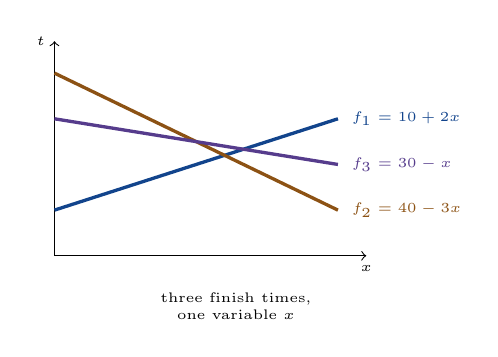
\begin{tikzpicture}[xscale=0.36, yscale=0.058, font=\tiny]
  \draw[->] (0,0) -- (11.0,0) node[below] {$x$};
  \draw[->] (0,0) -- (0,47) node[left] {$t$};
  \draw[very thick, ruleink] (0,10) -- (10,30);
  \draw[very thick, demoink] (0,40) -- (10,10);
  \draw[very thick, watchink] (0,30) -- (10,20);
  \node[ruleink, anchor=west] at (10.15,30) {$f_1 = 10 + 2x$};
  \node[demoink, anchor=west] at (10.15,10) {$f_2 = 40 - 3x$};
  \node[watchink, anchor=west] at (10.15,20) {$f_3 = 30 - x$};
  \node[align=center] at (6.4,-11) {three finish times,\\ one variable $x$};
\end{tikzpicture}
\hspace{7mm}
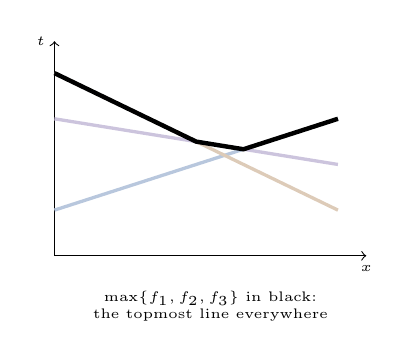
\begin{tikzpicture}[xscale=0.36, yscale=0.058, font=\tiny]
  \draw[->] (0,0) -- (11.0,0) node[below] {$x$};
  \draw[->] (0,0) -- (0,47) node[left] {$t$};
  \draw[very thick, ruleink!30] (0,10) -- (10,30);
  \draw[very thick, demoink!30] (0,40) -- (10,10);
  \draw[very thick, watchink!30] (0,30) -- (10,20);
  \draw[ultra thick, black] (0,40) -- (5,25) -- (6.667,23.33) -- (10,30);
  \fill (5,25) circle (1.6pt); \fill (6.667,23.33) circle (1.6pt);
  \node[align=center] at (5.5,-11) {$\max\{f_1, f_2, f_3\}$ in black:\\ the topmost line everywhere};
\end{tikzpicture}
\hspace{7mm}
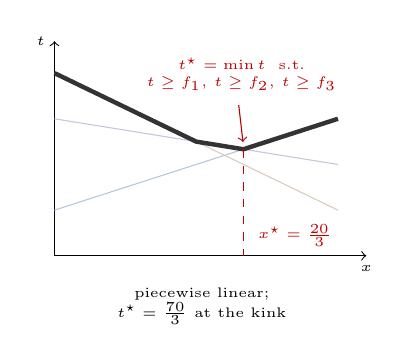
\begin{tikzpicture}[xscale=0.36, yscale=0.058, font=\tiny]
  \draw[->] (0,0) -- (11.0,0) node[below] {$x$};
  \draw[->] (0,0) -- (0,47) node[left] {$t$};
  \draw[ruleink!30] (0,10) -- (10,30);
  \draw[demoink!30] (0,40) -- (10,10);
  \draw[watchink!30] (0,30) -- (10,20);
  \draw[ultra thick, black!80] (0,40) -- (5,25) -- (6.667,23.33) -- (10,30);
  \draw[dashed, red!75!black] (6.667,23.33) -- (6.667,0);
  \fill[red!75!black] (6.667,23.33) circle (1.9pt);
  \node[red!75!black, anchor=west] at (6.85,4.5) {$x^{\star} = \tfrac{20}{3}$};
  \node[red!75!black, align=center, anchor=south] at (6.6,34)
    {$t^{\star} = \min t$ \ s.t.\\ $t \ge f_1,\, t \ge f_2,\, t \ge f_3$};
  \draw[->, red!75!black] (6.5,33) -- (6.65,24.9);
  \node[align=center] at (5.2,-11) {piecewise linear;\\ $t^{\star} = \tfrac{70}{3}$ at the kink};
\end{tikzpicture}
\end{center}
\vspace{3pt}

in general, worst-case objectives turn linear:
\[
  \min_{x}\; \max\bigl\{ f_1(x), \dots, f_k(x) \bigr\}
  \qquad\iff\qquad
  \begin{aligned}[t]
  \min_{x,\,t}\quad & t \\
  \text{s.t.}\quad & f_i(x) \le t \ \ \forall i \in [k]
  \end{aligned}
\]
$t$ sits above every $f_i$; min presses it onto the largest \ $\Rightarrow$ \ optimal $t$ $=$ the max.
\ linear $f_i$ $\Rightarrow$ an LP
\end{board}
\key{``minimize the worst case'' became linear rows --- the same move returns in weeks 9 and 13.}

% ---------------------------------------------------------------- 6
\beat{6}{Fixed costs --- paying to switch something on}
\begin{board}
open a site ($x \in \{0,1\}$, fixed cost $c$) before stocking $y \ge 0$ (cost $f$/unit):
\[
  \text{cost} \; = \; c\,x + f\,y, \qquad\quad
  y \;\le\; M x \qquad \text{(\textbf{linking constraint}, $M$ = ``big $M$'')}
\]
\quad $x = 0 \ \Rightarrow\ y = 0$ \qquad\quad closed site holds nothing
\vspace{1pt}

\quad $x = 1 \ \Rightarrow\ y \le M$ \qquad\ \ open site holds up to $M$
\end{board}
\key{``$y > 0$'' is not linear --- no LP can see it. the binary is the price of a discontinuity: $x$ lets linear constraints say \emph{if--then}.}

% ---------------------------------------------------------------- 7
\beat{7}{Logical conditions --- binaries as switches}
\begin{board}
yes/no $\leftrightarrow$ yes/no: plain inequalities, no $M$ --- check by trying the $0/1$ cases:
\vspace{3pt}

\begin{center}
\begin{tabular}{lll}
 ``if 1 is on, 2 must be on'' & {\footnotesize 1을 켜면 2도 켜야} & $x_1 \le x_2$ \\[2pt]
 ``1 or 2 --- at least one on (both fine)'' & {\footnotesize 1 또는 2 중 최소 하나 켬 (둘 다 가능)} & $x_1 + x_2 \ge 1$ \\[2pt]
 ``1 or 2 --- not both on (neither fine)'' & {\footnotesize 1 또는 2 중 최대 하나 켬 (둘 다는 불가)} & $x_1 + x_2 \le 1$ \\[2pt]
 ``either 1 or 2 --- exactly one on'' & {\footnotesize 1 또는 2 중 정확히 하나 켬} & $x_1 + x_2 = 1$ \\[2pt]
 ``at most $p$ of $n$ on'' & {\footnotesize $n$개 중 최대 $p$개 켬} & $\sum_{i \in [n]} x_i \le p$ \\[2pt]
 ``at least $p$ of $n$ on'' & {\footnotesize $n$개 중 최소 $p$개 켬} & $\sum_{i \in [n]} x_i \ge p$ \\[2pt]
 ``if 1 is on, then 2 or 3 is on'' & {\footnotesize 1을 켜면 2 또는 3도 켜야} & $x_1 \le x_2 + x_3$ \\[2pt]
 ``if 1 is on, then \emph{either} 2 or 3 is on'' & {\footnotesize 1을 켜면 2 또는 3 중 하나만 켜야} & $x_1 \le x_2 + x_3, \ \ x_2 + x_3 \le 2 - x_1$ \\[2pt]
 ``1 on: exactly one of 2, 3 on --- 1 off: both off'' & {\footnotesize 1 켜면 2$\cdot$3 중 하나만, 끄면 둘 다 끔} & $x_1 = x_2 + x_3$ \\
\end{tabular}
\end{center}
\vspace{4pt}

yes/no $\leftrightarrow$ \emph{continuous} constraint: \
\textbf{active} at $\bar y$: $a^{\top}\bar y = \beta$; \ \textbf{redundant}: deleting it changes nothing.
\ inflate the right side --- $M \ge \max_y (a^{\top}y - \beta)$ --- and any constraint goes redundant
\vspace{3pt}

\emph{redundant $=$ switched \textbf{off}} \ $\Rightarrow$ \ $M(1-x)$ makes $x$ a \textbf{switch}:
\[
  a^{\top}y \;\le\; \beta + M(1-x)
  \qquad
  \begin{cases}
    x = 1: & a^{\top}y \le \beta \quad \text{(enforced)}\\[2pt]
    x = 0: & \text{redundant --- off}
  \end{cases}
\]
\emph{example:} \ on the box $0 \le y_1 \le 100$, \ $0 \le y_2 \le 60$:
\quad $2y_1 + 3y_2 \;\le\; 6 + M(1-x)$
\vspace{1pt}

\quad smallest valid $M = \max_y\,(2y_1 + 3y_2) - 6
  = 2 \cdot 100 + 3 \cdot 60 - 6 = 374$ \quad --- each $y_j$ at its own worst bound
\begin{center}
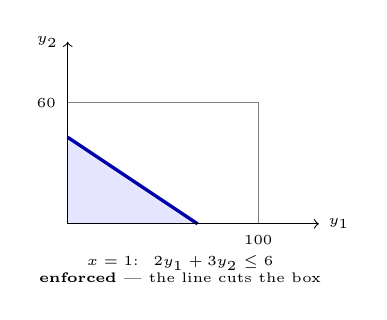
\begin{tikzpicture}[scale=0.55, font=\tiny]
  \fill[blue!10] (0,0) -- (3,0) -- (0,2) -- cycle;
  \draw[thin,gray] (0,0) rectangle (4.4,2.8);
  \draw[very thick, blue!65!black] (3,0) -- (0,2);
  \draw[->] (0,0) -- (5.8,0) node[right] {$y_1$};
  \draw[->] (0,0) -- (0,4.2) node[left] {$y_2$};
  \node[below] at (4.4,-0.05) {$100$};
  \node[left] at (-0.05,2.8) {$60$};
  \node[align=center] at (2.6,-1.05) {$x = 1$: \ $2y_1 + 3y_2 \le 6$\\ \textbf{enforced} --- the line cuts the box};
\end{tikzpicture}
\hspace{12mm}
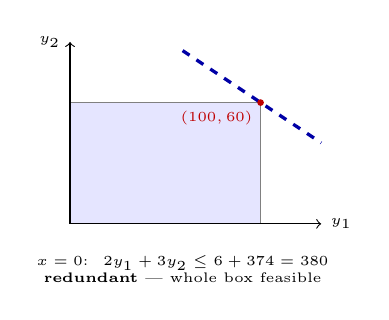
\begin{tikzpicture}[scale=0.55, font=\tiny]
  \fill[blue!10] (0,0) rectangle (4.4,2.8);
  \draw[thin,gray] (0,0) rectangle (4.4,2.8);
  \draw[very thick, blue!65!black, dashed] (2.6,4.0) -- (5.8,1.87);
  \fill[red!75!black] (4.4,2.8) circle (2.2pt);
  \node[red!75!black, anchor=north east, inner sep=1.5pt] at (4.32,2.72) {$(100,60)$};
  \draw[->] (0,0) -- (5.8,0) node[right] {$y_1$};
  \draw[->] (0,0) -- (0,4.2) node[left] {$y_2$};
  \node[align=center] at (2.6,-1.05) {$x = 0$: \ $2y_1 + 3y_2 \le 6 + 374 = 380$\\ \textbf{redundant} --- whole box feasible};
\end{tikzpicture}
\end{center}
activating the big-$M$ term slides the line out of the box --- and with the
\emph{smallest} valid $M$ it rests exactly on the far corner $(100,60)$: any smaller
$M$ would still cut the box (WRONG --- next section). \ \emph{sketches not to scale}
\vspace{3pt}

\textbf{either--or} \ (a union --- not convex, no LP describes it):
\[
  a_1^{\top}y \le b_1 + M(1-x), \qquad a_2^{\top}y \le b_2 + M x, \qquad x \in \{0,1\}
\]
\textbf{at least $k$ of $m$}: \ one switch each, $k$ switches on:
\[
  a_i^{\top}y \;\le\; b_i + M(1 - x_i) \quad \forall i \in [m], \qquad
  \textstyle\sum_{i \in [m]} x_i \;\ge\; k
\]
\vspace{2pt}

\textbf{minimum load} \ airlift $y_1$ ($0 \le y_1 \le 80$) flies in bulk or not at all:
\ $y_1 = 0$ \ OR \ $y_1 \ge 50$
\vspace{2pt}

write it in the either--or form --- one switch:
\[
  y_1 \;\le\; 0 + M(1-x), \qquad
  -y_1 \;\le\; -50 + M x, \qquad x \in \{0,1\}
  \qquad (M = 80 \ \text{works: } y_1 \le 80)
\]
\quad check: \ $x = 1$: $y_1 \le 0$ enforced, the $\ge 50$ row off; \qquad
$x = 0$: $y_1 \ge 50$ enforced, the $\le 0$ row off
\vspace{4pt}

\textbf{2 of 3 criteria} \ stockpile ($y_1$ fuel, $y_2$ ammo, $y_1 + y_2 \le 50$);
certify if 2 of: \ total $y_1 + y_2 \ge 40$, \quad fuel $y_1 \ge 25$, \quad ammo $y_2 \ge 25$
\vspace{2pt}

flip each $\ge$ to $\le$, one switch per criterion, at least $k = 2$ on:
\[
  -y_1 - y_2 \;\le\; -40 + M(1-x_1), \qquad
  -y_1 \;\le\; -25 + M(1-x_2), \qquad
  -y_2 \;\le\; -25 + M(1-x_3)
\]
\[
  x_1 + x_2 + x_3 \;\ge\; 2, \qquad x \in \{0,1\}^3
  \qquad (M = 40,\, 25,\, 25 \ \text{suffice: with } y \ge 0 \text{ each ``off'' row is redundant})
\]
\quad check: \ $x = (1,1,0)$: total and fuel enforced, the ammo row off --- any two on $\Rightarrow$ certified
\end{board}
\demo{demo2c\_logical\_constraints.py}{``at least $k$ of 3'' on a box --- the feasible set is visibly a non-convex union.}
\key{one idea: big-$M$ makes a constraint redundant on demand --- a binary becomes a switch. either--or, $k$-of-$m$, if--then: the same switch, different wiring.}

% ---------------------------------------------------------------- 8
\beat{8}{How big should $M$ be?}
\begin{board}
\textbf{too small: WRONG.} \ the ``off'' constraint still cuts feasible plans --- the solver silently
returns the best plan \emph{of the wrong problem}
\vspace{3pt}

\textbf{too large: WEAK.} \ $x = 0.01$, $M = 10^5$ already unlocks $y \le 1000$ ---
bound far from truth, solver slow
\vspace{3pt}

the craft: the \textbf{smallest certainly-valid $M$} --- a physical quantity (budget, demand, capacity), never $10^6$
\end{board}
% ---------------------------------------------------------------- next
\enlargethispage{4\baselineskip}
\par\medskip
{\color{ruleink}\rule{\textwidth}{1.2pt}}\par\nobreak\vspace{3pt}
{\color{keyink}\small\textbf{next lecture}\quad the binary capstone (best-subset selection), matching --- and the classic IP models: assignment, transportation, \emph{total unimodularity}. \ \textbf{Homework 1 is out} (due week 4).}

\end{document}
